%&tex

\chapter{Object Shape Learning}\label{sec:shapelearning}
% \begin{comment}

	% PENN SHAPES
	\begin{figure}[htp]
		\begin{subfigure}{1.\textwidth}
		\centering
		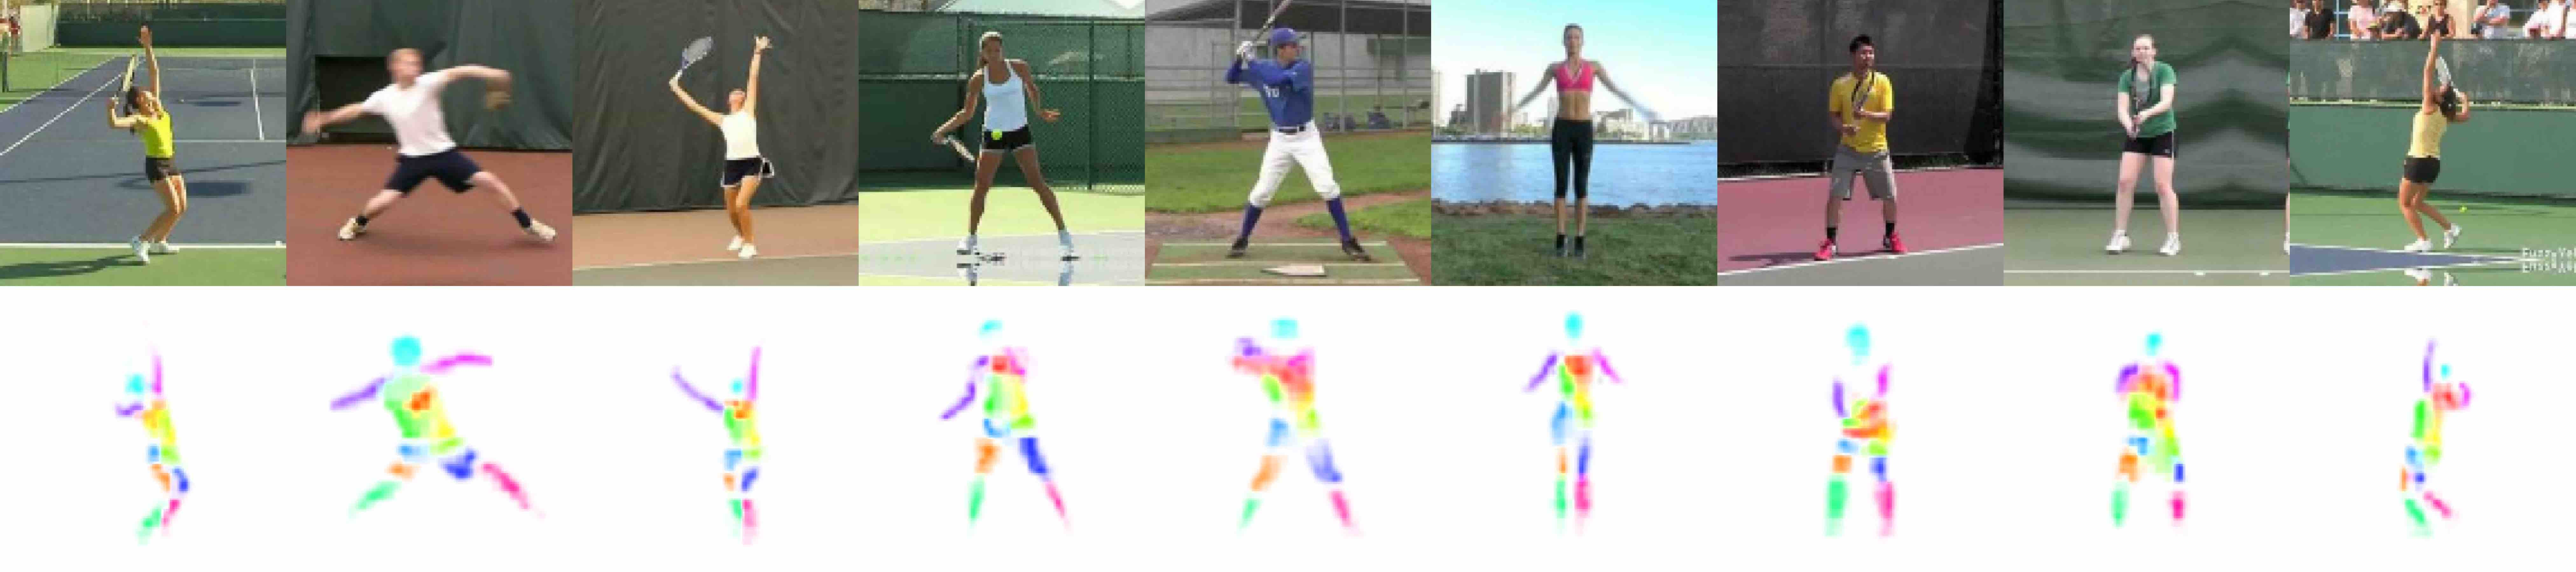
\includegraphics[trim={0cm 0cm 0cm 0cm},clip, width=1.\linewidth]{fig/shape/shape8white}\caption{}
		\label{fig:shape_penn}
		\end{subfigure}
		\begin{subfigure}{1.\textwidth}
		\centering
		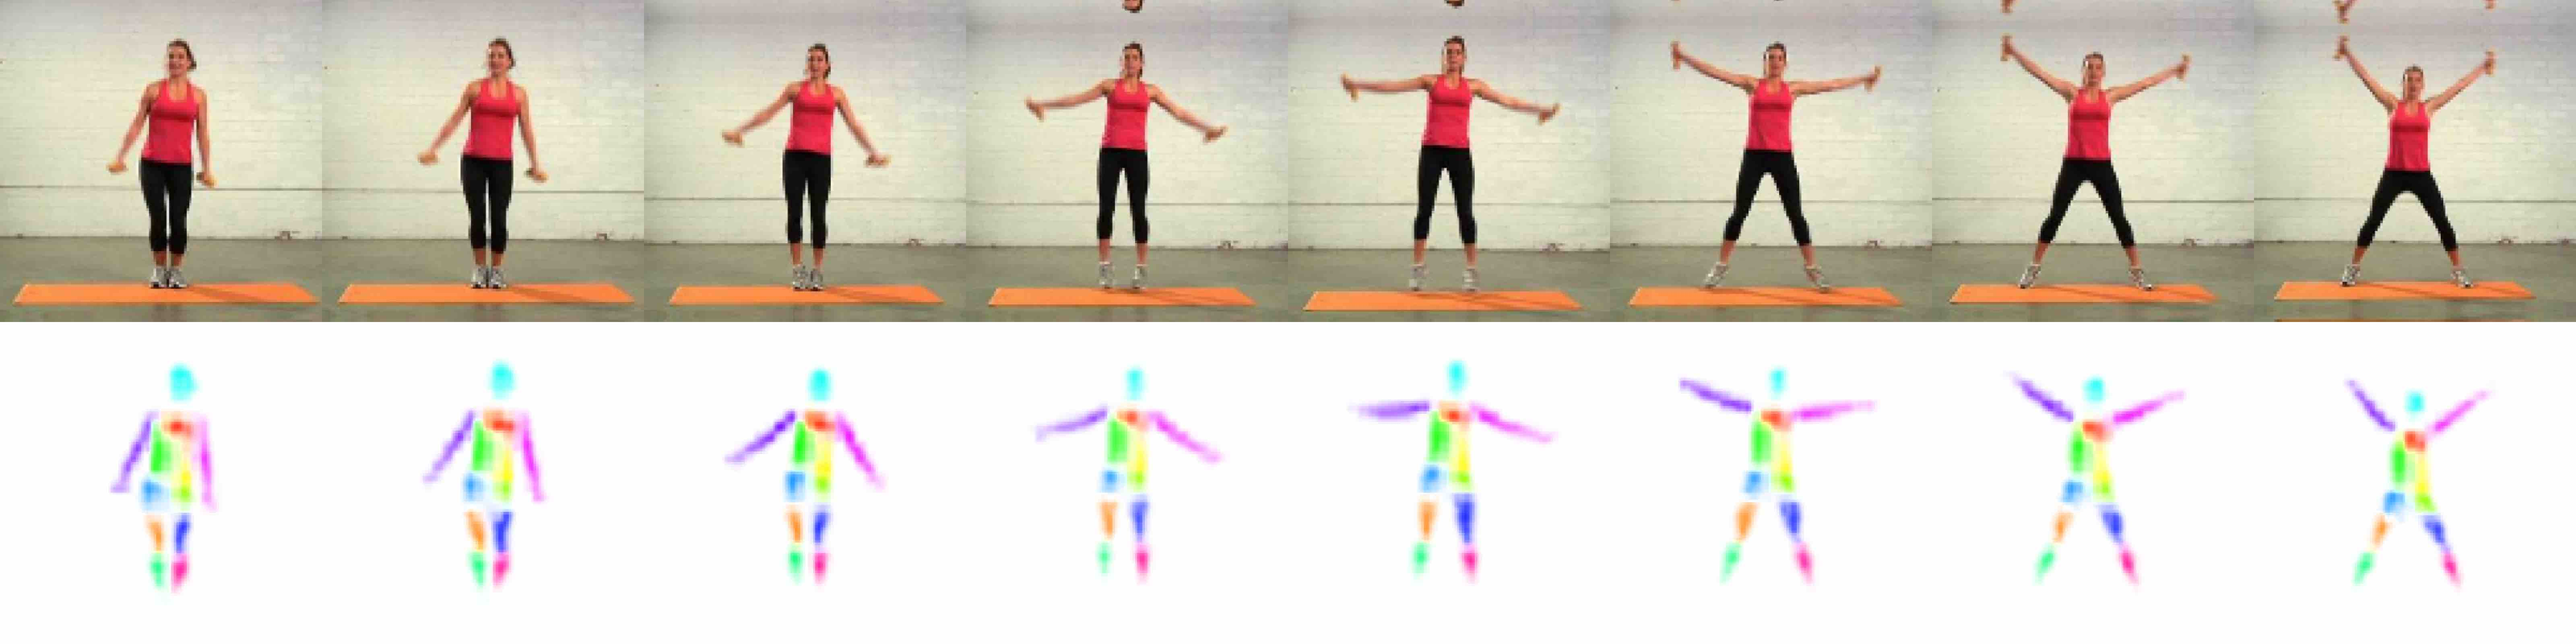
\includegraphics[trim={0cm 0cm 0cm 0cm},clip, width=1.\linewidth]{fig//shape/shape_yoga8}\caption{}
		\label{fig:shape_tennis}
		\end{subfigure}
		\caption{Learned shape representation on Penn Action. For visualization, 13 of 16 part activation maps are plotted in one image. (a) Different instances, showing intra-class consistency and (b) video sequence, showing consistency and smoothness under motion, although each frame is processed individually.}
		\label{fig:shapespenny}
	\end{figure}

	In this section we will establish that the proposed method (Chapter~\ref{sec:method}) outperforms the state-of-the-art in unsupervised object shape learning by a large margin.
	The learned shape representation is visualized in Fig.~\ref{fig:shapespenny}. \todo{ours region-based, landmarks only for evaluation}
	To quantitatively evaluate the shape estimation, we measure how well groundtruth landmarks (only during testing) are predicted from it.
	We obtain landmarks from our part-region based shape representation by designating the mean of a part shape $\mu[\sigma^i(\mathbf{x})]$ as the landmark position. To quantify the quality of these landmark estimates, we linearly regress them to human-annotated groundtruth landmarks and measure the test error.
	% The part shape means $\mu[\sigma^i(x)]$ serve as our landmark estimates and we measure the error when linearly regressing the human-annotated groundtruth landmarks from these estimates.
	For this, we follow the protocol of Thewlis \etal \cite{thewlis17}, fixing the network weights after training the model, extracting unsupervised landmarks and training a single linear layer without bias.
	The performance is quantified on a test set by the mean error and the percentage of correct landmarks (PCK).
	We extensively evaluate our model on a diverse set of datasets, each with specific challenges.
	% On all datasets we outperform the state-of-the-art by a significant margin.


	In the following, we proceed through our shape learning results: we present the quantitative and qualitative {results} by object category (Sec.~\ref{sec:results}).
	On the way we introduce the datasets for each category.
	In the next section we highlight and discuss the challenges, which the datasets present (Sec.~\ref{sec:challenges}) and subsequently argue for the importance of the transformations and modelling assumptions  as a means to reach disentanglement and to overcome those challenges (Sec.~\ref{sec:transformations}).
	This confirms that disentangled modelling aids the learning of shape (Hypothesis I, Sec.~\ref{sec:contributions}).

\section{Diverse Object Categories}\label{sec:results}
	% On the object classes of human faces, cat faces, and birds and human and animal bodies our model predicts landmarks consistently across different instances.
	We test our approach on a diverse set of object classes ranging from human and cat faces to articulated bodies and animals. In the following we go through the results sorted by object category. Where possible we compare to state-of-the-art methods quantitatively in terms of unsupervised landmark prediction, additionally we show qualitative results.
	\subsection{Human and Cat Faces}\label{sec:kp_faces}
		% FACES
		\begin{figure}[htp]
			\centering
			\begin{subfigure}{1.\textwidth}
			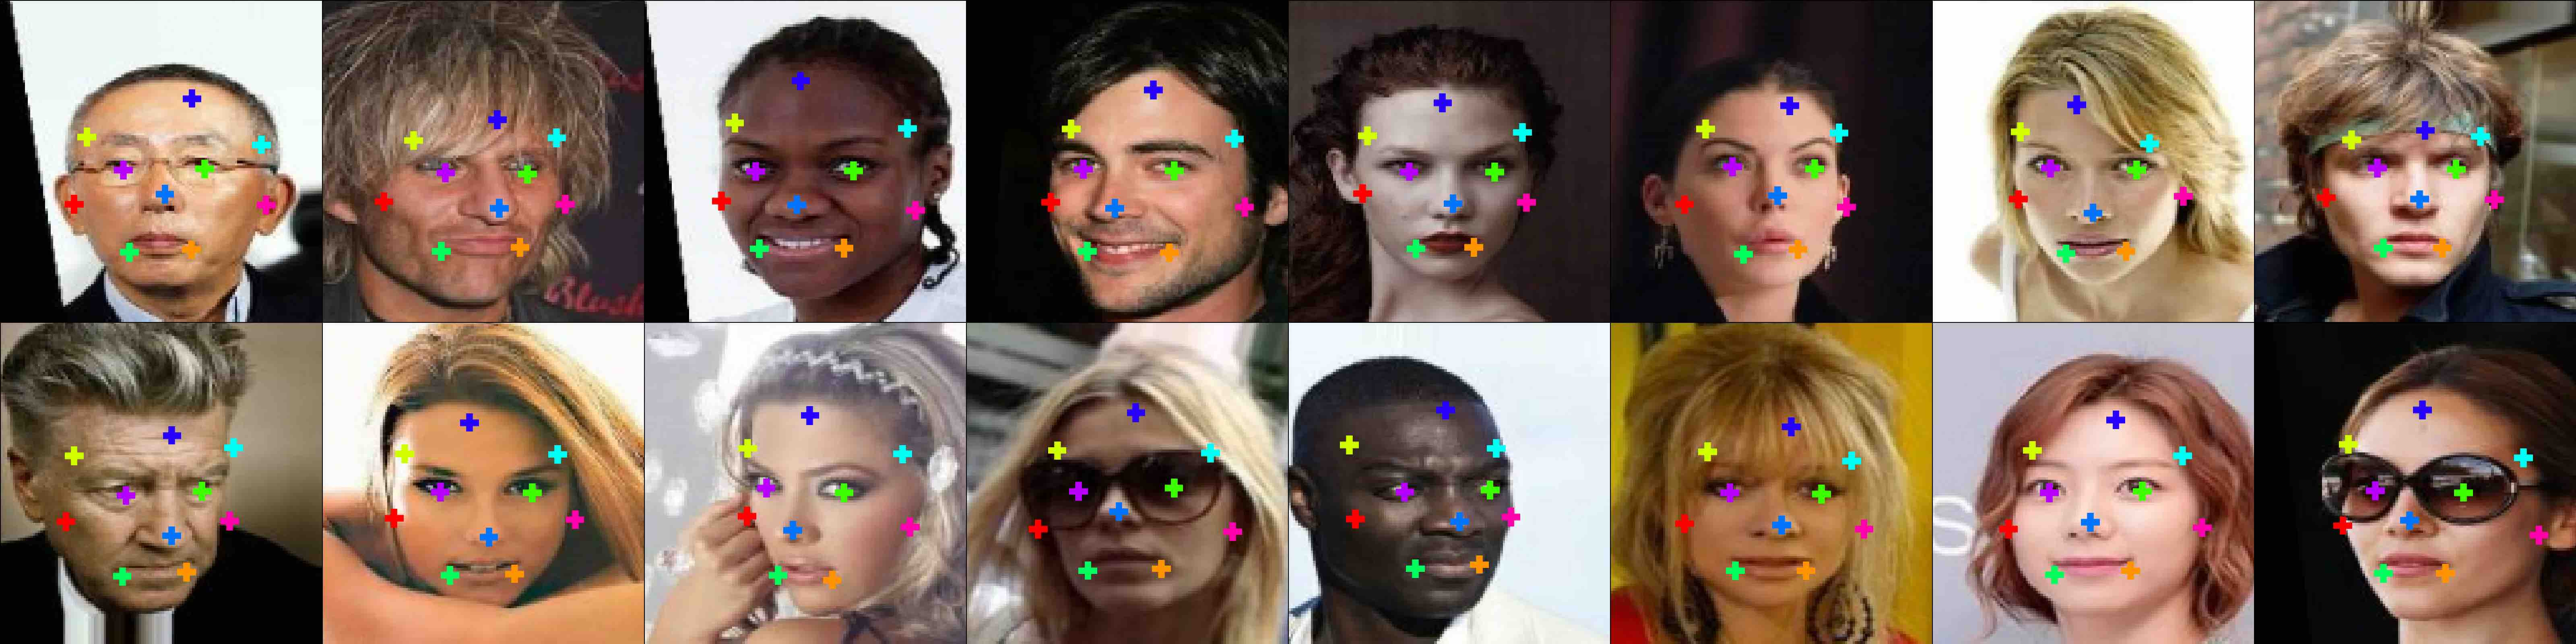
\includegraphics[trim={0cm 0cm 0cm 0cm},clip, width=1.\linewidth]{fig/shape/0celeba}\caption{}
			\end{subfigure}
			\begin{subfigure}{1.\textwidth}
			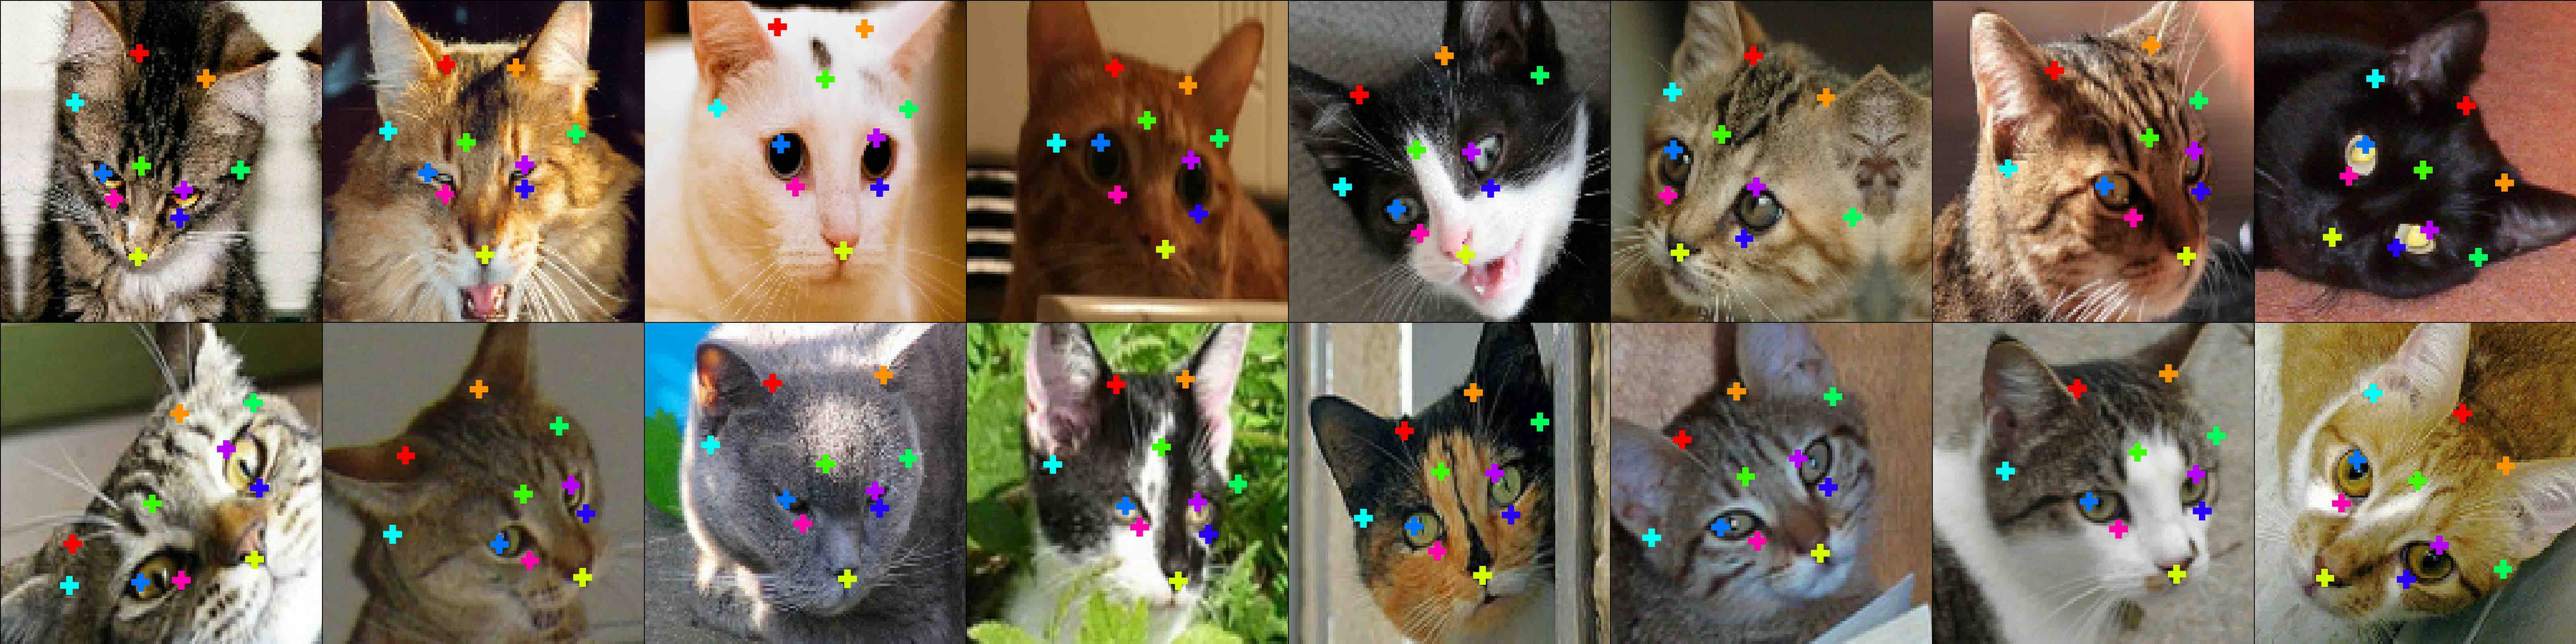
\includegraphics[trim={0cm 0cm 0cm 0cm},clip, width=1.\linewidth]{fig/shape/0cats}\caption{}
			\end{subfigure}
			\caption{{Unsupervised discovery of landmarks the object classes of (a) human (CelebA dataset) and (b) cat faces (Cat Head dataset).}}
			\label{fig:kp_faces}
		\end{figure}

		% \subsubsection{Dataset preprocessing}
		For human and cat faces we use the popular datasets CelebA and Cat Head, since our predecessors for unsupervised shape learning established baselines here. Both object categories are rather rigid and non-articulated - meaning that the relations between object parts are not changing from instance to instance.
		Due to different breeds, the Cat Head dataset exhibits large variations between instances. Cat faces feature more complicated texture and locally variant silhouettes \cite{zhang08cathead}, hence, require a better learning of both shape and appearance.

			\begin{tcolorbox}
				\textbf{CelebA} \cite{liu15facewild} contains ca. 200k celebrity faces of 10k identities.
				We resize all images to $128\times 128$ and exclude the training and test set of the MAFL subset, following \cite{thewlis17}.
				As  \cite{thewlis17, zhang18}, we train the regression (to 5 ground truth landmarks) on the MAFL training set (19k images) and test on the MAFL test set (1k images).
			\end{tcolorbox}

			\begin{tcolorbox}
				\textbf{Cat Head} \cite{zhang08cathead}  has nearly 9k images of cat heads.
				We use the train-test split of \cite{zhang18} for training (7,747 images) and testing (1,257 images).
				We regress 5 of the 7 (same as \cite{zhang18}) annotated landmarks.
				The images are cropped by bounding boxes constructed around the mean of the ground truth landmark coordinates and resized to $128\times128$.
			\end{tcolorbox}

		\subsubsection{Qualitative results}
			The algorithm successfully defines correspondences between different human individuals, and also generalizes between different cat breeds.
			On both datasets the performance is visibly near-perfect.
			Difficulties such as out-of-plane rotation, varying lighting conditions and part occlusions (\eg sunglasses) do not diminish its ability to determine the self-defined keypoints.


		\subsubsection{Quantitative results}
			% RESULTS FACES
			\begin{table}[t]
				\caption{Error of unsupervised methods for landmark prediction on the Cat Head, MAFL (subset of CelebA) testing sets. The error is in \% of inter-ocular distance.}
				\label{tab:faces}
				\centering
				\begin{tabular}{l|ccc}
				\hline
				Dataset & Cat Head &  & MAFL \\
				  \# Landmarks &10 & 20  & 10  \\
				  \hline
				 Thewlis \etal \cite{thewlis17}
				 & 26.76 & 26.94 & 6.32    \\
				 Jakab \etal \cite{jakab18}
				 & - & - & 4.69  \\
				 Zhang \etal \cite{zhang18}
				 & 15.35 & 14.84 & 3.46  \\
				  Ours & \textbf{9.88}  & \textbf{9.30} & \textbf{3.24}  \\ \hline  % image length is 600: 32.15 , 23.51
				\end{tabular}
			\end{table}
			Tab.~\ref{tab:faces} compares against the state-of-the-art.
			Our approach outperforms competing methods, with a particularly large margin of ca. $4-5\%$ on the more challenging Cat Head dataset. The best competitor suffers from an incomplete disentanglement (as we show in Sec.~\ref{sec:zhang}).
			Here we observed, that the most severe failure modes for the Cat Head dataset were human labelling errors, which suggests that the unsupervised performance could be better than the human labelling under these circumstances.

	\subsection{Human Bodies}\label{sec:kp_humanbodies}
		% BODIES
		\begin{figure}[htp]
			\centering
			\begin{subfigure}{1.\textwidth}
			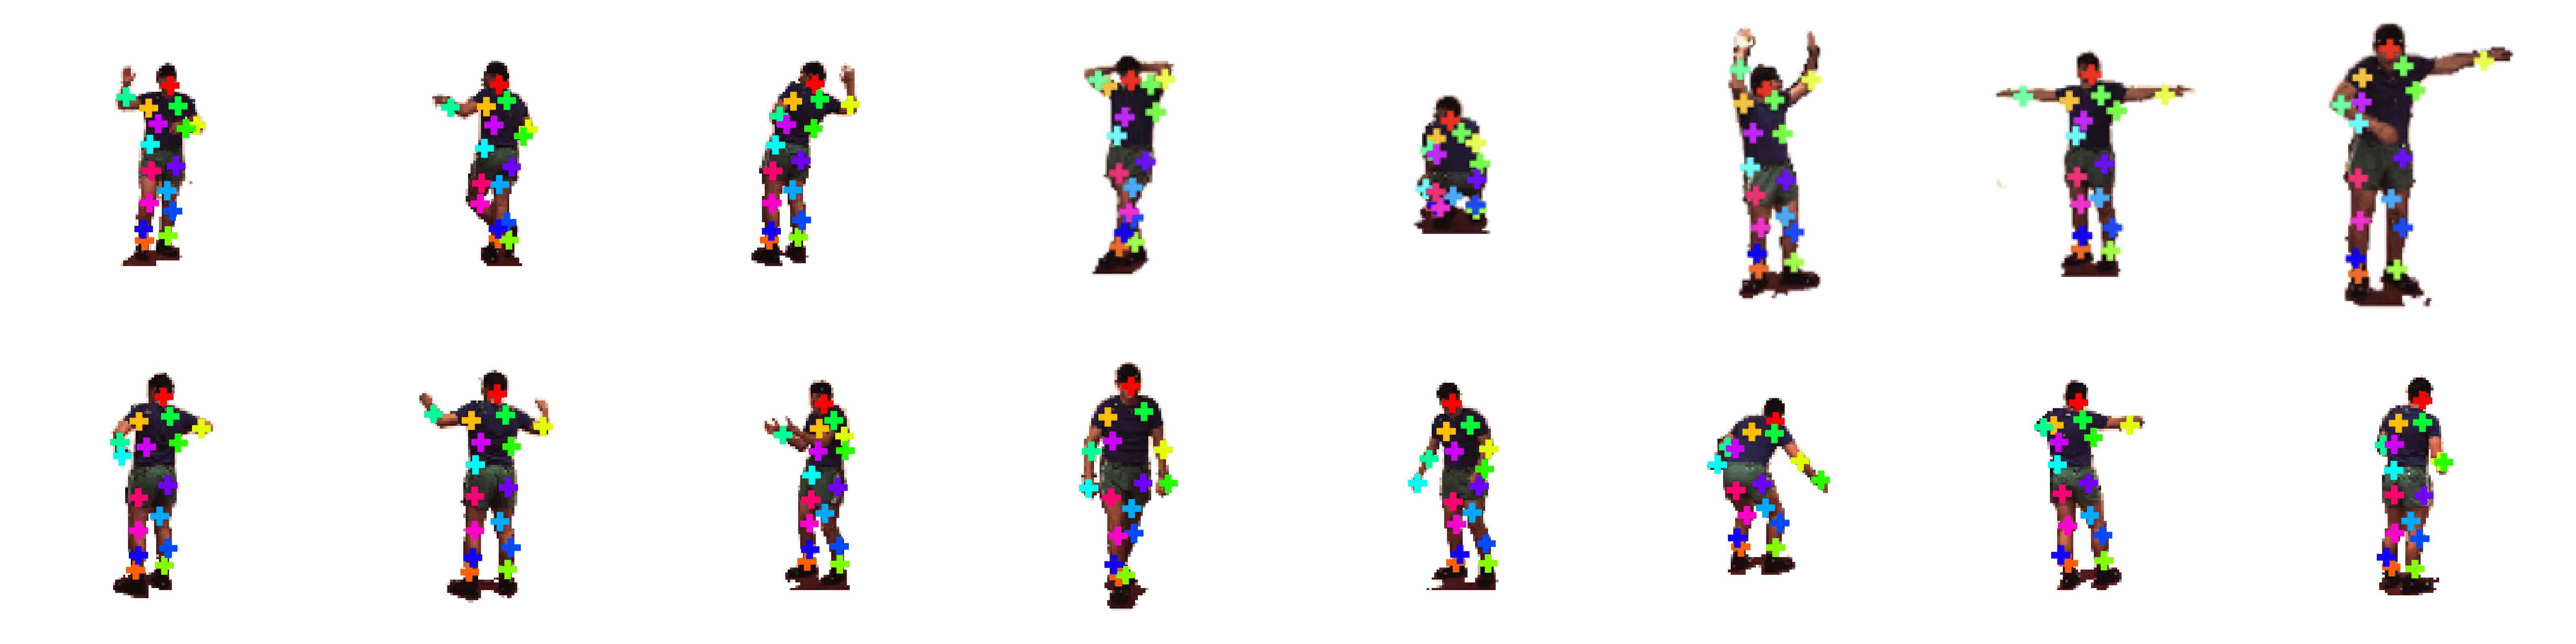
\includegraphics[trim={0cm 0cm 0cm 0cm},clip, width=1.\linewidth]{fig/shape/0human}\caption{}
			\end{subfigure}
			\begin{subfigure}{1.\textwidth}
			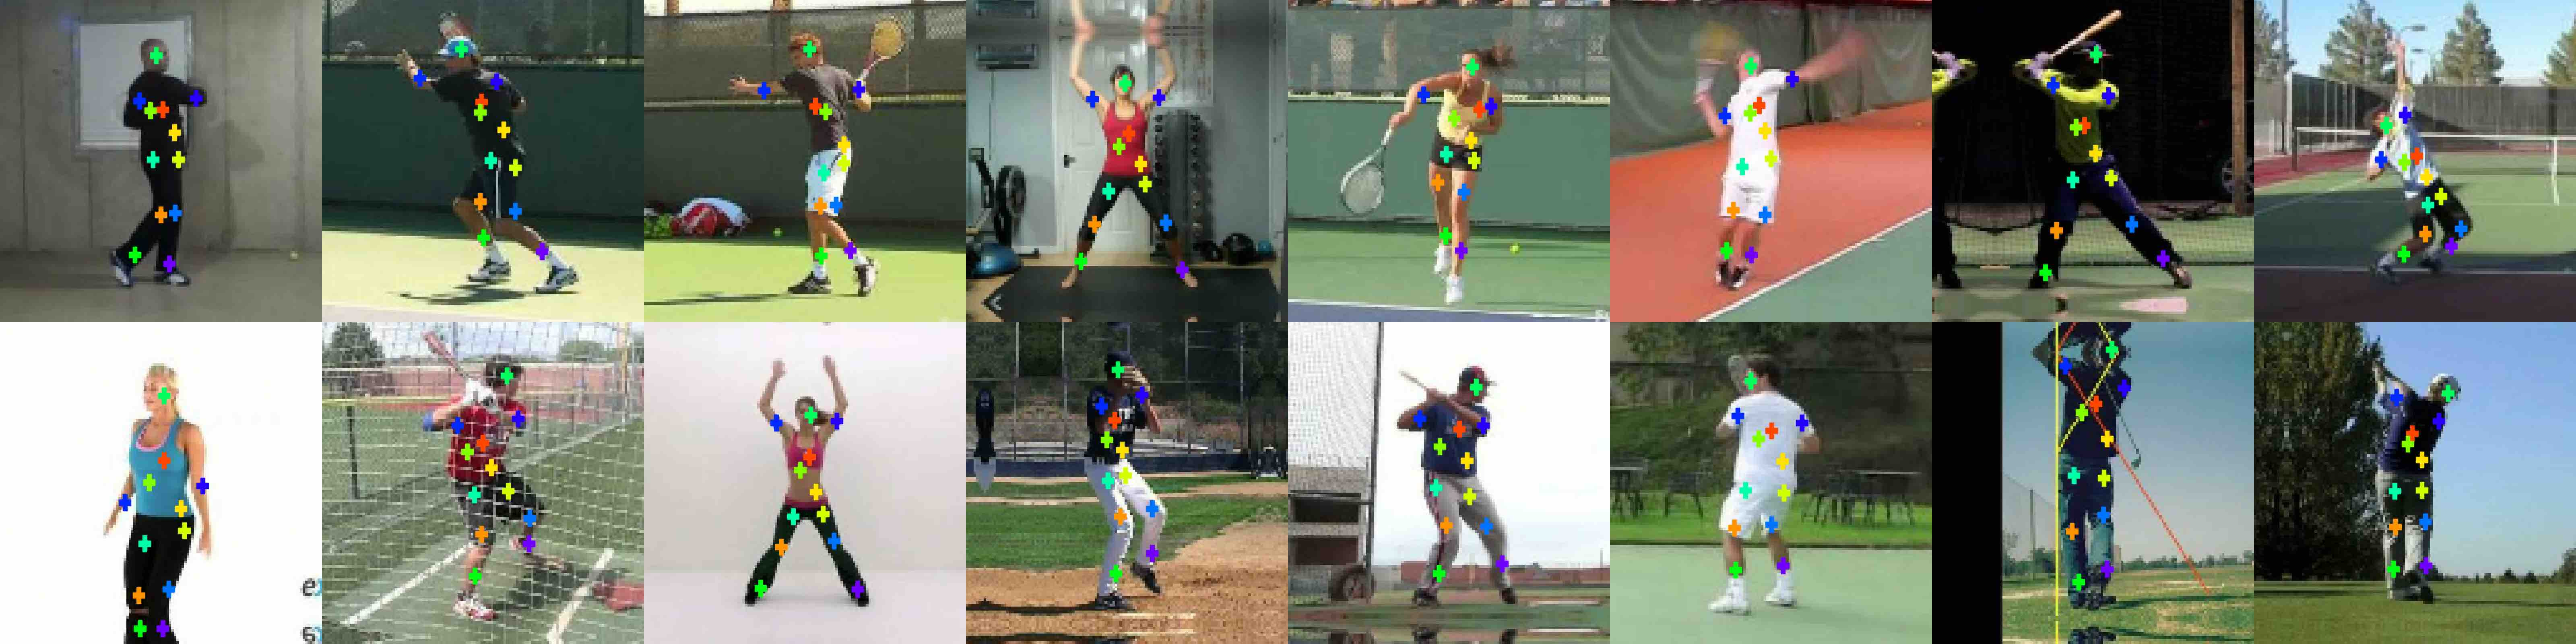
\includegraphics[trim={0cm 0cm 0cm 0cm},clip, width=1.\linewidth]{fig/shape/0penn}\caption{}
			\end{subfigure}
			\caption{{Unsupervised discovery of landmarks the object classes of human bodies (a) in constrained (Human3.6M dataset) and (b) unconstrained environments (Penn Action dataset).}}
			\label{fig:kp_bodies}
		\end{figure}

		Human bodies introduce the challenge of object articulation. We test on three datasets. The BBC Pose dataset is used to compare against Jakab \etal~\cite{jakab18}, the Human3.6M dataset to beat the benchmark of Zhang \etal~\cite{zhang18}. Additionally, we present the first unsupervised results on Penn Action, which is, as we argue, significantly more difficult.
		% In contrast to the considerable pose variation, the appearance variation among the 7 subjects is limited due to the lighting conditions and similar clothing.
		% Penn Action: In contrast to both BBC Pose and Human3.6M both pose and appearance variation is huge, real-world conditions.

			\begin{tcolorbox}
				\textbf{BBC Pose} \cite{charles13bbcpose} contains videos of sign-language signers with varied appearance in front of a changing background.
				The test set includes 1000 frames and the test set signers did not appear in the train set.
				Like \cite{jakab18} we loosely crop around the signers: we used image patches measuring $300 \times 300$ pixels, which we resized to a resolution of $128 \times 128$.
				For evaluation, as \cite{jakab18}, we utilized the provided evaluation script, which measures the PCK around $d=6$ pixels in the original image resolution.
			\end{tcolorbox}
			\begin{tcolorbox}
				\textbf{Human3.6M} \cite{ionescu14human36m} features human activity videos in stable environments. We consider a subset of ca. 800k images from 6 activities (direction, discussion, posing, waiting, greeting, walking).
				We adopt the training and evaluation procedure of \cite{zhang18}: We trained on 6 subjects IDs (S1, S5, S6, S7, S8, S9) and used S11 for testing.
				For proper comparison to \cite{zhang18} we also removed the background using the off-the-shelf unsupervised background subtraction method provided in the dataset and cropped roughly around the provided bounding boxes, then resized to $128 \times 128$.
				For evaluation, as~\cite{zhang18}, we report the minimum of the errors to the original landmark annotations and their left-right-flipped counterparts. This is correcting for the fact, that the model does not distinguish back and frontal views (for a discussion of this problem, cf. Sec.~\ref{sec:parity}).
			\end{tcolorbox}
			\begin{tcolorbox}
				\textbf{Penn Action} \cite{zhang13penn} contains 2326 video sequences of 15 different sports categories.
				For this experiment we use 6 categories (tennis serve, tennis forehand, baseball pitch, baseball swing, jumping jacks, golf swing).
				We roughly cropped the images around the person, using the provided bounding boxes, then resized to $128\times128$.
			\end{tcolorbox}

		\subsubsection{Qualitative results}
			We demonstrate (Fig. \ref{fig:kp_bodies}), that our model not only exhibits strong landmark consistency under articulation, but also covers the full human body meaningfully.
			Even fine-grained parts such as the arms are tracked across heavy body articulations, as are present in the Human3.6M or Penn Action datasets.
			Also with further complications introduced with the Penn Action dataset such as viewpoint variations, blurred limbs and partial self-occlusions we are able to detect landmarks of similar quality and coverage as in the more constrained Human3.6M dataset.
			Additionally, complex background clutter, as in BBC Pose and Penn Action, does not hinder finding the object.

		\subsubsection{Quantitative results}

			The quantitative comparisons are shown in Tab.~\ref{tab:bbcpose} and Tab.~\ref{tab:human}: other unsupervised and semi-supervised methods are outperformed by a large margin on both datasets.

			On Human3.6M, judging by the performance gap, it is questionable whether the other unsupervised method from Thewlis \etal~\cite{thewlis17} learned to deal with articulation at all or whether they just find a mean solution.We beat the best unsupervised result by Zhang \etal~\cite{zhang18} by an improvement of $2.12\%$. This is not only cutting the absolute error nearly in half, but also reduces the gap between unsupervised and supervised algorithms by about $77\%$.
			Zhang \etal~\cite{zhang18} additionally used optical flow to stabilize their training by forcing the landmarks to cover the object, which we (and they themselves) classified as semi-supervised.
			Despite this advantage, our approach is able to achieve a performance gain of $1.35\%$ even over results obtained with optical flow supervision.  %The  relative position and errors of our landmarks compared to the manually annotated landmarks are shown in Fig. \ref{fig:regress}.

			On BBC Pose, we outperform Jakab \etal~\cite{jakab18} by $6.1\%$, which translates into a reduction of the unsupervised performance gap to supervised methods by more than half. An analysis of conceptual differences to both~\cite{zhang18} and~\cite{jakab18} can be found in Sec.~\ref{sec:compare}.

			% BBC POSE Results
			\begin{table}[htp]
				\caption{{
				Performance of landmark prediction on BBC Pose test set. As upper bound, we also report the performance of supervised methods.
				%Comparing against supervised and unsupervised methods for annotated landmark prediction on the BBC Pose testing set.
				The metric is \% of points within 6 pixels of groundtruth location. %Note that Jakab et al. are using a 50-landmarks, while we only use a 30 landmarks as input for the regression.
				}}
				\label{tab:bbcpose}
				\centering
				\begin{tabular}{ll|cr}
				\hline
				BBC Pose &   &    { Accuracy}  \\
				 \hline
				supervised & Charles \etal \cite{charles13bbcpose} &
				   79.9\%  \\ % 79.90
				 & Pfister \etal \cite{pfister15flowingconv}  &
				  88.0\%  \\ \hline % 88.01
				unsupervised &Jakab \etal \cite{jakab18} &
				 68.4\%  \\  % 68.44
				  &Ours &  \textbf{74.5}\% \\
				% test pck = 0.7484605918670523
				% test pck_per_kp = [0.9633621  0.6627155  0.76508623 0.54956895 0.6928879  0.76616377   0.83943963]
				\hline
				\end{tabular}
			\end{table}

			% HUMAN3.6M Results
			\begin{table}[htp]
				\caption{{Comparing against supervised, semi-supervised and unsupervised methods for landmark prediction on the Human3.6M test set. The
				error is in \% of the edge length of the image. All methods predict 16 landmarks.
				}}
				\label{tab:human}
				\centering
				\begin{tabular}{ll|cr}
				\hline
				 Human3.6M   & &  { Error w.r.t. image size}  \\
				 \hline
				 supervised & Newell \etal \cite{newell16hourglass}
				  &2.16  \\  \hline
				 semi-supervised & Zhang \etal \cite{zhang18}
				  & 4.14  \\ \hline
				 unsupervised & Thewlis \etal \cite{thewlis17}
				 & 7.51  \\
				  & Zhang \etal \cite{zhang18}
					& 4.91 \\
				  & Ours& \textbf{2.79} \\
				\hline
				\end{tabular}
			\end{table}




	\subsection{Animal Bodies}\label{sec:kp_animalbodies}
		% DOGS, BIRDS
		\begin{figure}[htp]
			\centering
			\begin{subfigure}{1.\textwidth}
			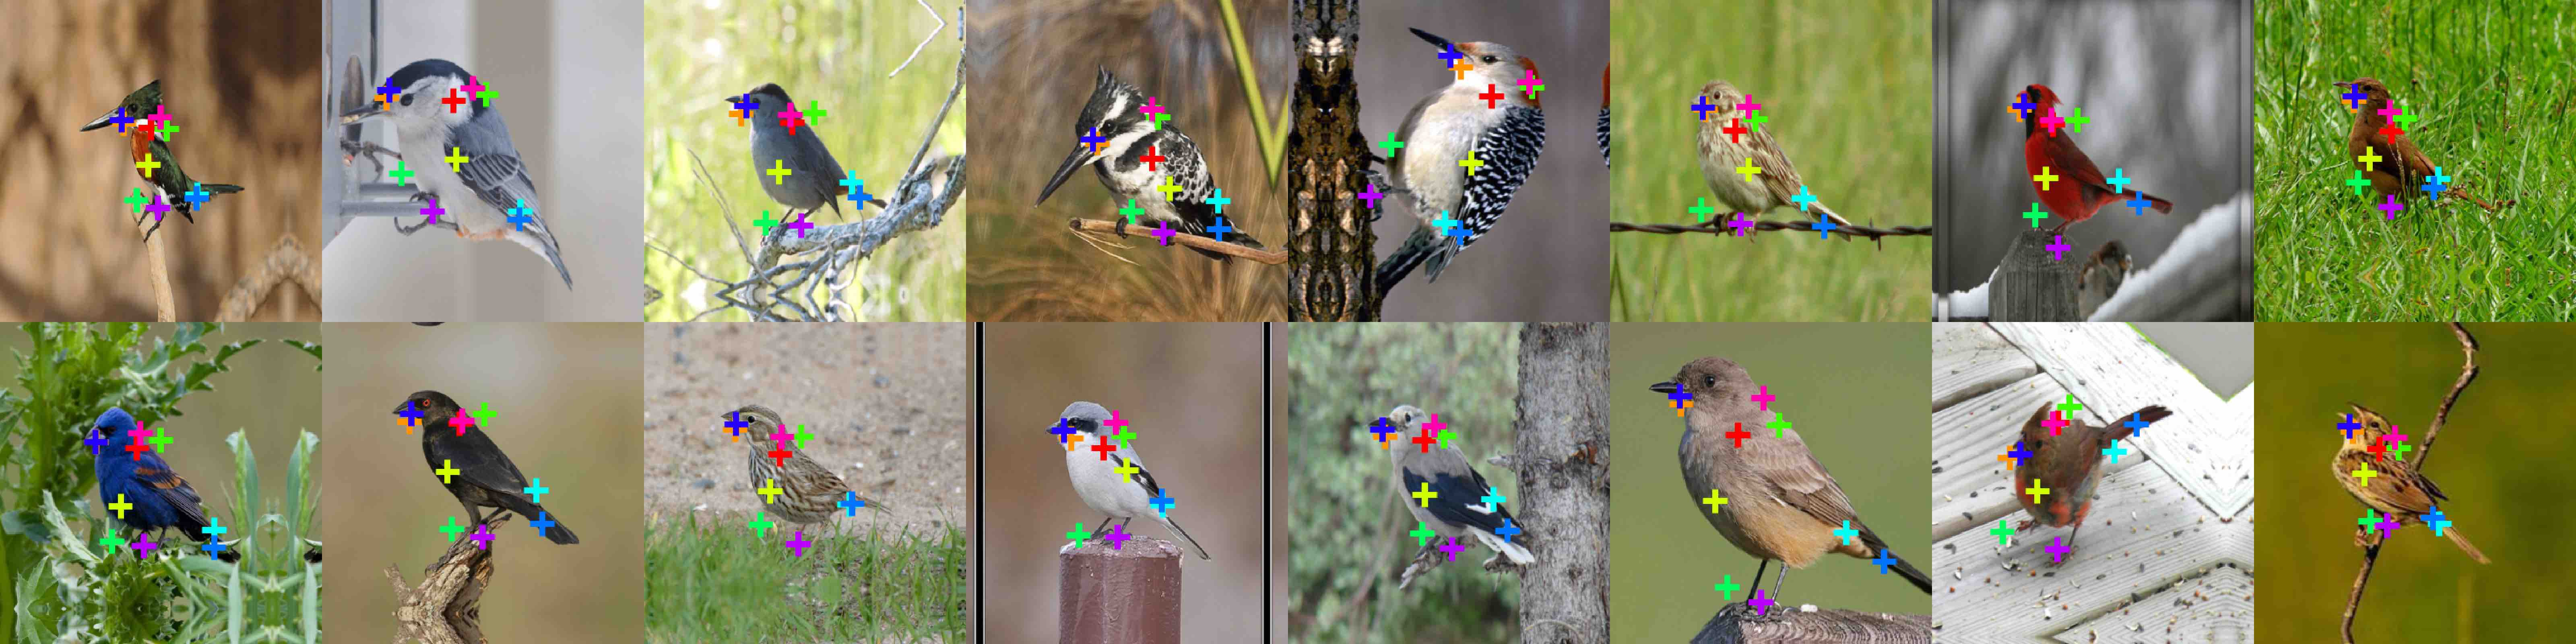
\includegraphics[trim={0cm 0cm 0cm 0cm},clip, width=1.\linewidth]{fig/shape/0birds}\caption{}
			\end{subfigure}
			\begin{subfigure}{1.\textwidth}
			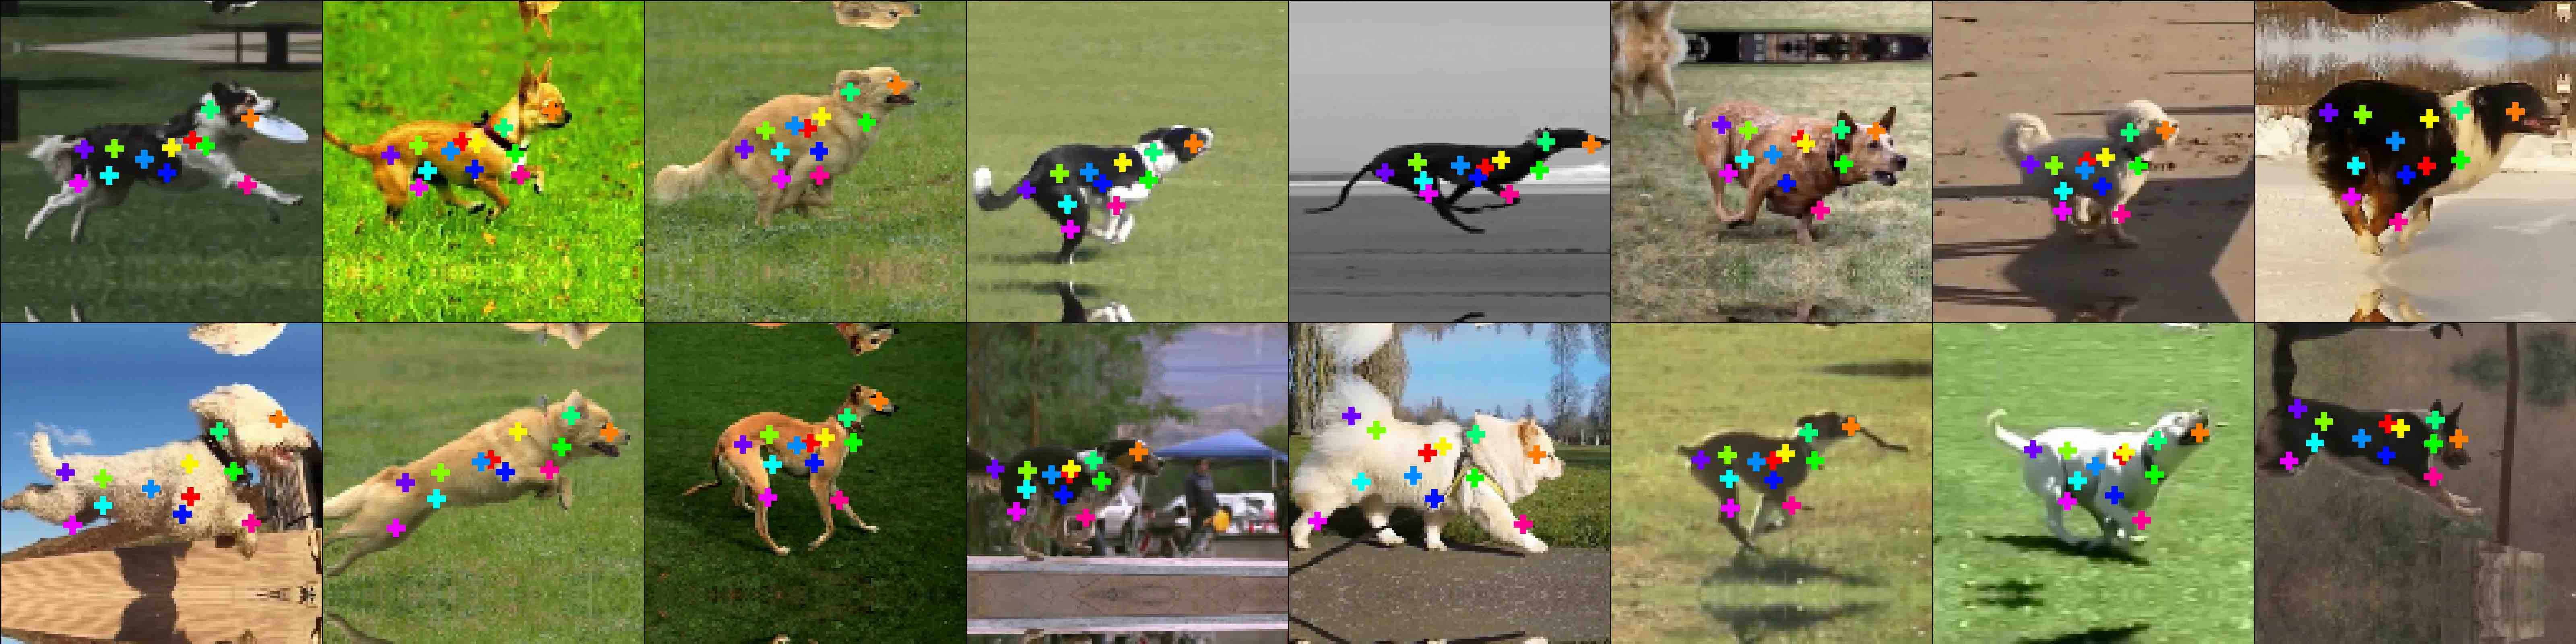
\includegraphics[trim={0cm 0cm 0cm 0cm},clip, width=1.\linewidth]{fig/shape/0dogs}\caption{}
			\end{subfigure}
			\caption{{Unsupervised discovery of landmarks the object classes of animal bodies (a) birds (CUB-200-2011 dataset) and (b) dogs (Dogs Run dataset).}}
			\label{fig:kp_animals}
		\end{figure}

		% \subsubsection{Dataset preprocessing}

		\begin{tcolorbox}
			\textbf{CUB-200-2011} \cite{wah11birds} comprises ca. 12k images of birds in the wild from 200 bird species.
			% flying birds impossible because transition information missing
			We excluded bird species of seabirds, because these bird species were depicted flying, (discussion in Sec.~\ref{sec:articulation}), roughly cropped using the provided landmarks as bounding box information and resized to $128\times128$.
			We aligned the parity with the information about the visibility of the eye landmark (discussion in Sec.~\ref{sec:parity}).
			For comparing with \cite{zhang18} we used their published code.
		\end{tcolorbox}
		\begin{tcolorbox}
			\textbf{Dogs Run} is made from dog videos from YouTube totaling in 1250 images under similar conditions as in Penn Action. The dogs are running in one direction in front of varying backgrounds. The 17 different dog breeds exhibit widely varying appearances.
		\end{tcolorbox}

		\subsubsection{Qualitative results}
			On CUB-200-2011 the model discovers consistent landmarks that closely cover the bird's body, despite significant variation in color, texture, size and background. The direct comparison to Zhang \etal~\cite{zhang18} is further discussed in Sec.~\ref{sec:compare}, including a qualitative comparison in Fig.~\ref{fig:compare}.
			The performance on the Dogs Run dataset shows that highly differing dog breeds (size, thickness of fur) can be related via semantic parts.
			Furthermore, the limited amount of data in Dogs Run is no problem for finding meaningful correspondences, due to the unsupervised nature of the model and the transformations acting as a form of data augmentation.
			On both datasets, the universality of the approach (capturing non-human poses) is underlined once more.
			This is to be expected, as no specific assumptions about the object-class are introduced in the model formulation.


		\subsubsection{Quantitative results}

			For a direct comparison to Zhang \etal \cite{zhang18} we apply their published code on the CUB-200-2011 dataset. The results are shown in Tab.~\ref{tab:birds}. Our method surpasses~\cite{zhang18}; to appreciate why this is so, refer to the direct comparison in Sec.~\ref{sec:zhang}.


			% RESULTS BIRDS
			\begin{table}[t]
				\caption{Error of unsupervised methods for landmark prediction on the CUB-200-2011 testing set. Both methods predict 10 landmarks.}
				% The error is in \% of edge length of the image.}
				\label{tab:birds}
				\centering
				\begin{tabular}{l|cccc}
					\hline
					CUB-200-2011 dataset&  & Error \wrt image edge\\
					% \# Landmarks & 10  \\
					\hline
					Zhang \etal \cite{zhang18} & 5.36 \\
					Ours  & \textbf{3.91}  \\ \hline
				\end{tabular}
			\end{table}


\section{Overcoming Challenges}\label{sec:challenges}
	%DATASET CHALLENGES
	\begin{table}[htp]
		\centering
		\caption{Difficulties of datasets: articulation, intra-class variance, background clutter and viewpoint variation}
		\label{tab:challenges}
		\begin{tabular}{l|rrrr}
			\hline
			Dataset &  Articulation & Intra-Class &  Background & Viewpoint \\ \hline
			CelebA &   &  &  &    \\
			Cat Head & &  \checkmark&  &   \\
			CUB-200-2011 & & \checkmark& \checkmark&   \\
			Human3.6M &\checkmark& &  & \checkmark  \\
			BBC Pose &  \checkmark&  & \checkmark&  \\
			Dogs Run & \checkmark& \checkmark& \checkmark&   \\
			Penn Action & \checkmark& \checkmark& \checkmark& \checkmark  \\
			\hline
		\end{tabular}
	\end{table}
	An overview over the challenges implied by each of the presented datasets is given in Tab.~\ref{tab:challenges}. We address the main difficulties in the following: background clutter~\ref{sec:background}, intra-class variance~\ref{sec:intraclass}, articulation and viewpoint variation~\ref{sec:articulation}.
	We make suggestions on how the method overcomes these challenges.

	\subsection{Background Clutter}\label{sec:background}
		The question how to separate background from object goes deeper than one might think. Fundamentally the question is equivalent to: \textit{What is an object?}
		If an unsupervised algorithm is given the task of finding the object in an image dataset - under the assumption that the object is present in all images - the object is a structure common to these images.
		By this definition background is everything that is not strongly correlated with the object itself.
		This dataset-specific object category can be unintuitive: for example for a bird sitting on a twig, the twig can be considered as part of the object (\eg two landmarks are on feet/twig on CUB-200-2011 dataset,  cf. Fig.~\ref{fig:kp_animals}).
		This dataset-biased pre-categorical thinking of unsupervised algorithms can be seen as a failure, or as a feature: on a dataset of dancing humans our method identified the pair of dancers as the salient object (cf. Fig.~\ref{fig:parity}). \todo{better figure here, make salsa dataset}
		Technically, we allow the algorithm to focus on the reconstruction of only the object, and not background by a local weighting around the part activation (refer to Sec.~\ref{sec:implementationdetails}). The fundamental issue of strong object-background correlations might not be solved technically, but require different data or prior knowledge. \todo{look up (and reference to) dataset bias} Interestingly, on with the constrained but repetitive background of the Human3.6M dataset, where traditional background subtraction methods are easily applied, our method struggles: several parts are assigned to background objects. On the other hand, complexly cluttered backgrounds - as long as no correlations to the object exist - such as the background TV screen in the BBC Pose dataset (cf. Fig.~\ref{fig:bbcthumb}) are actually favorable for the method. This is due to the crossed reconstruction objective: if reconstructing the background of the target image is possible with the information of the source appearance image, the algorithm will try to do so by assigning parts to the background, if not, not.


		\subsection{Object Articulation and Viewpoint Variation}\label{sec:articulation}

		Object articulation and viewpoint variation makes consistent shape learning challenging. In contrast to rigid bodies that can vary in orientation and scale, articulated objects have many degrees of freedom more. Viewing from different points increased the difficulty both in the rigid and the articulated case.
		Complex articulation can be conceptually simplified by regarding an object as a collection of rigid parts, that again each have only few degrees of freedom. This description of an arrangement of parts is exponentially cheaper than trying to capture it as a whole~\cite{ross06parts}. To enforce the factorization into independent parts it is crucial to restrain the part features and region to be local (how exactly is shown in Sec.~\ref{sec:method}). Landmarks are a simple and efficient implementation of this part factorization idea. In this sense, using landmarks as shape representation is the natural approach for tackling articulation. However, related work does not strictly enforce locality of the learned features (compare~\ref{sec:jakab}) or a local reconstruction from these features.


		Part assignment consistency means equivariance \wrt changes in shape due to articulation. Equivariance is enforced twice in the method (cf. Sec.~\ref{sec:framework}).
		We showed previously that the method can deal with strongly articulated human and animal bodies (cf. Sec.~\ref{sec:kp_humanbodies} and Sec.~\ref{sec:kp_animalbodies}).
		\todo{Viewpoint variation, cnns bad at viewpoint}
		% no grid -> Zhang
		% % ill-posed fundamentally if reconstruction, cf.\ bbcpose to see that from trainset possible.
		\todo{discuss about shape transformation, for which no transformation present, like birds flying, deep fashion leg crossing.}

	\subsection{Intra-Class Variation}\label{sec:intraclass}
		Intra-class variation can be both in shape and in appearance. Due to different breeds and species the animal datasets - Dogs Run, CUB-200-2011, Cat Head - present the highest degree of variability within the object class. The method in part coincidentally generalizes and in part inherently enforces in due to the data augmentation with shape and appearance transformations (see also Sec. \ref{sec:transformations}).

\section{Comparative Advantages}\label{sec:compare}
		In this section we directly compare against the closest competitors on unsupervised learning of shape Zhang \etal~\cite{zhang18} and Jakab \etal~\cite{jakab18}. On a low-level, there are many differences to both approaches, some of which we discuss in the respective related work (Sec.~\ref{sec:relshapelearning}). On a high level, the main difference is that Zhang \etal lacks a principled way to disentangle shape and appearance (\eg via transformations) (Sec.~\ref{sec:zhang}) and Jakab \etal models the appearance in a holistic encoding (Sec.~\ref{sec:jakab}).

		\subsection{Non-Disentangling Approach}\label{sec:zhang}
			% HUMAN3.6M DETAILED RESULTS
			\begin{table}[!ht]
				\centering
				\begin{tabular}{l|cccccr}
				\hline
				Dataset & Human3.6M  &  &  & &  &  \\
				Actions &  {\footnotesize Directions} & {\footnotesize Discussion} &  {\footnotesize Waiting }& {\footnotesize Greeting }& {\footnotesize Posing} & {\footnotesize Walking} \\
				\hline
				Newell \cite{newell16hourglass} (supervis.) %& 2.16
					& 1.88 & 1.92 & 2.15 & 1.62 & 1.88 & 2.21 \\
				Zhang \cite{zhang18}  (semi-superv.) %& 4.14
					& 5.01 & 4.61 & 4.76 & 4.45 & 4.91 & 4.61 \\  \hline
				Thewlis \cite{thewlis17}  (unsuperv.) % & 7.51
					& 7.54 & 8.56 & 7.26 & 6.47 & 7.93 & 5.40 \\
				Ours (unsuperv.) %& \textbf{2.79}
					& \textbf{2.58} & \textbf{2.26} & \textbf{2.87} & \textbf{3.08} & \textbf{2.67} & \textbf{3.35}\\
				\hline
				\end{tabular}
				\caption{{Comparison with unsupervised, semi-supervised and supervised methods for annotated landmark prediction on the Human 3.6M testing sets for selected actions. The
				error is in \% regarding the edge length of the image. All methods predict 16 landmarks, from which the 32 ground truth landmarks are regressed.}}
				\label{tab:humanactions}
			\end{table}

			% COMPARE ZHANG
			\begin{figure}[htp]
				\centering
				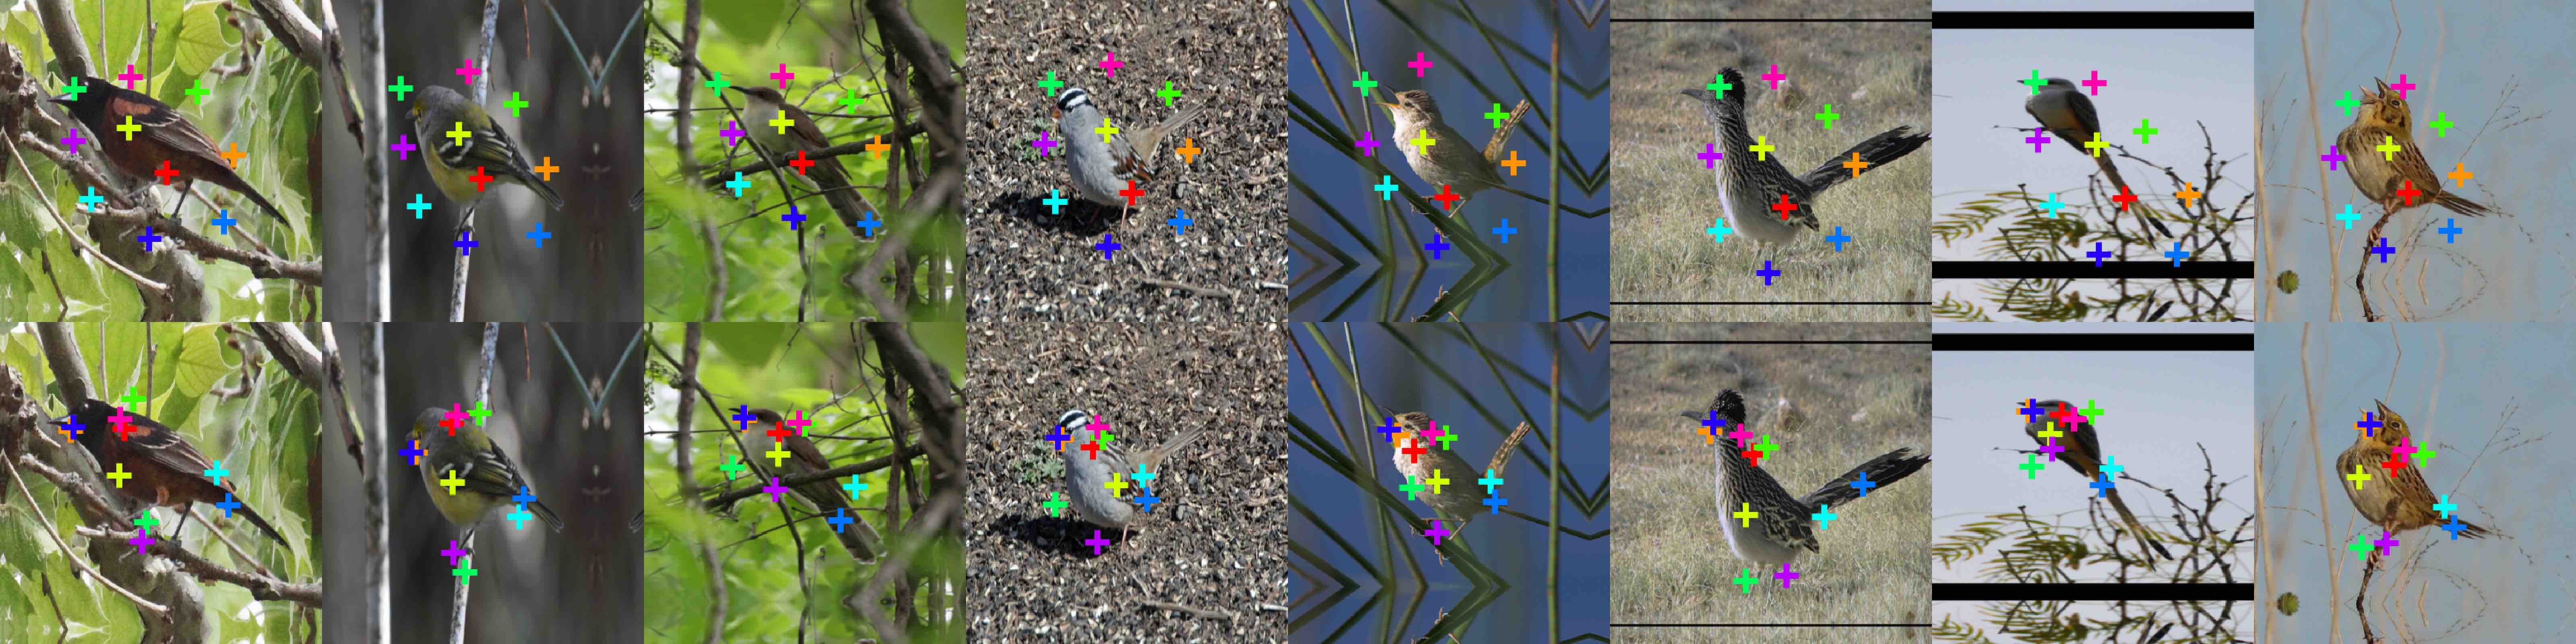
\includegraphics[trim={0cm 0cm 0cm 0cm},clip, width=1.\linewidth]{fig/shape/comp}
				\caption{Comparing discovered keypoints against \cite{zhang18} on CUB-200-2011. We improve on object coverage and landmark consistency. Note our flexible part placement compared to a rather rigid placement of \cite{zhang18} due to their part separation bias.}
				\label{fig:compare}
			\end{figure}

			The method of Zhang \etal \cite{zhang18} is similar to our method, but does not disentangle shape from appearance.
			\note{Zhang similar, but not disentangling, why does that fail, why do we succeed?}
			In Tab.~\ref{tab:humanactions} we list the detailed results of a comparison to Zhang \etal~\cite{zhang18}.
			Fig. \ref{fig:compare} provides a direct visual comparison to \cite{zhang18} on CUB-200-2011.\todo{reference table}
			It becomes evident that our predicted landmarks track the object much more closely.
			In contrast, \cite{zhang18} have learned a slightly deformable, but still rather rigid grid.
			This is due to their separation constraint, which forces landmarks to be mutually distant.
			We do not need such a problematic bias in our approach, since the localized, part-based representation and reconstruction guides the shape learning and captures the object and its articulations more closely.

		\subsection{Holistic Approach}\label{sec:jakab}
			The method of Jakab \etal \cite{jakab18} aims at disentangling shape and appearance with video information. Shape is then - similar to ours - defined by the change between consecutive frames. However, they do not model the link between local parts of shape and appearance, but use a holistic appearance embedding.
			% Constrained by reality.
			% \begin{itemize}
				% \item not factorizing into parts, holistic appearance
				% \item disentangle via video
				% \item particularly good on wrists, (highly articulated parts)
			% \end{itemize}

			% BBCPOSE DETAILED RESULTS
			\begin{table}[htp]
				\centering
				\begin{tabular}{l|ccccccr}
				\hline
				Dataset & BBC Pose &  &  &  & &  &  \\
				Landmarks & {\footnotesize Head} & {\footnotesize Wrists} &  {\footnotesize Elbows }& {\footnotesize Shoulders } & {\footnotesize Avg.}  \\
				\hline
				Charles \etal \cite{charles13bbcpose}  (supervised)&
				95.40 & 72.95 & 68.70 & 90.30 & 79.90  \\
				Pfister \etal  \cite{pfister15flowingconv} (supervised) &
				98.00 & 88.45 & 77.10 & 93.50 & 88.01  \\ \hline
				Jakab \etal \cite{jakab18}  (unsupervised) &
				76.10& 56.50& 70.70& 74.30 &68.44  \\
				Ours (unsupervised)  & \textbf{96.34} & \textbf{71.39} & \textbf{62.12} & \textbf{80.28}& \textbf{74.85} \\
				% test pck = 0.7484605918670523
				% test pck_per_kp = [0.9633621  0.6627155  0.76508623 0.54956895 0.6928879  0.76616377   0.83943963]
				\hline
				\end{tabular}
				\caption{{Comparison with supervised and unsupervised methods for annotated landmark prediction on the BBC Pose testing sets.
				\%-age of points within 6 pixels of ground-truth is reported.}}
				\label{tab:gtregressionhuman}
			\end{table}

			 % COMPARISON TO JAKAB
			\begin{figure}[htp]
				\centering
				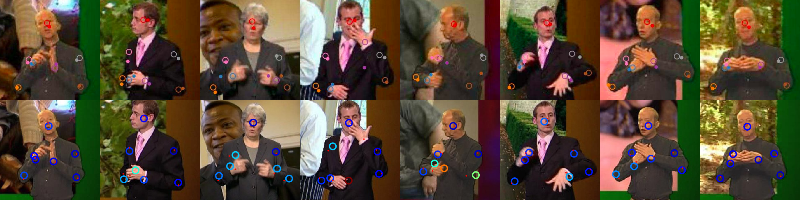
\includegraphics[trim={0cm 0cm 0cm 0cm},clip, width=1.\linewidth]{fig/shape/bbc8}
				\caption{Comparison of regression results of our method (bottom rows) to \cite{jakab18} (top rows) on BBC Pose. For visualization by Jakab \etal (from their paper) ground truth is in circles and the corresponding regression in the same color. For our visualization the red dots mark the ground truth, the colored circles the regressed locations. The color coding is in terms of the error \wrt the image edge length.}
				\label{fig:bbc8}
			\end{figure}
			\todo{color coding problem, reference to our regression figure}


	% \subsection{Failure Modes}\label{sec:failuremodes}
		\todo{search for failure modes}
		% on cat head, human mislabelling is the most common failure mode
	% background keypoints
	% discuss "overfitting" what does that even mean? - @domili


	\subsection{Ablating Contributions}\label{sec:ablation}
			% ABLATION STUDY
			\begin{table}
				\centering
				\begin{tabular}{l|cr}
					\hline
					Dataset & Cat Head    \\
					\# Landmarks &  20 \\ \hline
					full model &  9.30 \\ \hline
					w/o $\mathcal{L}_{\textrm{equiv}}$   & 11.32 \\
					w/o $\mathcal{L}_{\textrm{rec}}$   & 35.0 \\
					w/o appearance transform & 12.46 \\
					w/o shape transform & 14.72 \\ \hline
				\end{tabular}
				\caption{{Ablation studies on Cat Head dataset. We ablate the reconstruction loss $\mathcal{L}_{\textrm{rec}}$, equivariance loss $\mathcal{L}_{\textrm{equiv}}$, the color augmentation and the transformations}}
				\label{tab:ablation}
			\end{table}

			% what is the color augmentation: explain before
			\todo{what is the crossing task}
			Probably the most insightful comparison for a method is, to compare to lesser versions of itself.
			We ablate the main components of our proposed framework: reconstruction loss $\mathcal{L}_{\textrm{rec}}$, the equivariance loss $\mathcal{L}_{\textrm{equiv}}$, the appearance augmentation and the transformations for disentangling shape and appearance. For the ablation study we use the Cat Head dataset, following the already introduced train-test setup on the task of landmark ground truth regression. Tab. \ref{tab:ablation} illustrates the ablation results.\\
			Leaving out the reconstruction task naturally leads to the largest drop in performance, since training only on equivariance leads to collapsed landmark solutions as discussed in \cite{zhang18}.
			Note that without both shape and appearance transformations our models performs significantly worse, now comparable to Zhang \etal \cite{zhang18}.
			Without transformations the reconstruction objective is identical to the one of~\cite{zhang18}, only the model architecture deviates.
			This suggests, that the improved disentanglement (by transformations) could be explaining the overall performance gain \wrt \cite{zhang18}.  %This performance drop would be larger on datasets with articulation.
			Leaving out the explicit equivariance leads to the smallest drop in performance. This is not surprising, as equivariance is implicitly also enforced in the feature crossing in the framework.
			% without local features (not done yet, should we?, could ablate local decoder, or part appearance)



\section{Transformational Effects}\label{sec:transformations}
		% \note{in this section: effect of transformations on learning, disentangling}
		% \note{effectively connecting samples from the dataset, spreading the}
		\note{schedule transformations with exponential, formula}
		\note{as data augmentation}
		% \note{as blurring of data points}


		\begin{figure}[htp]
			\begin{subfigure}{0.40\linewidth}
				\centering
				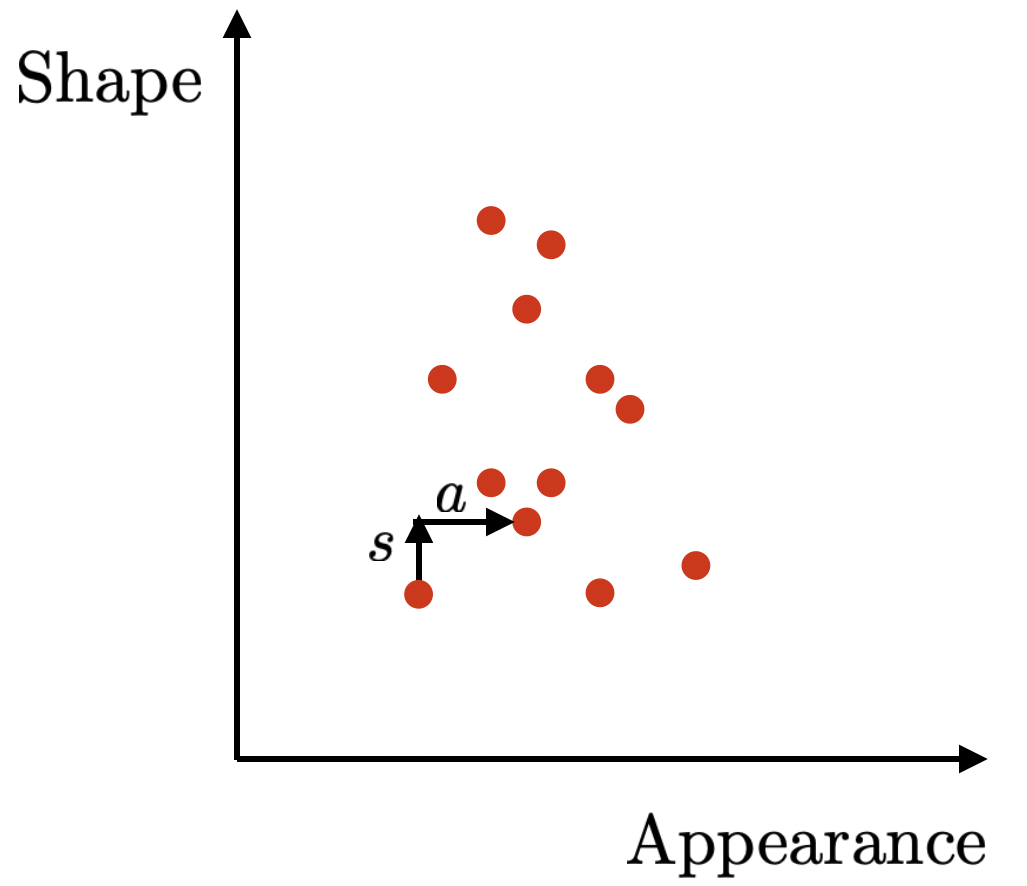
\includegraphics[trim={0cm 0cm 0cm 0cm},clip, width=1.\linewidth]{fig/other/trans}
				\caption{}
			\end{subfigure}
			\begin{subfigure}{0.40\linewidth}
				\centering
				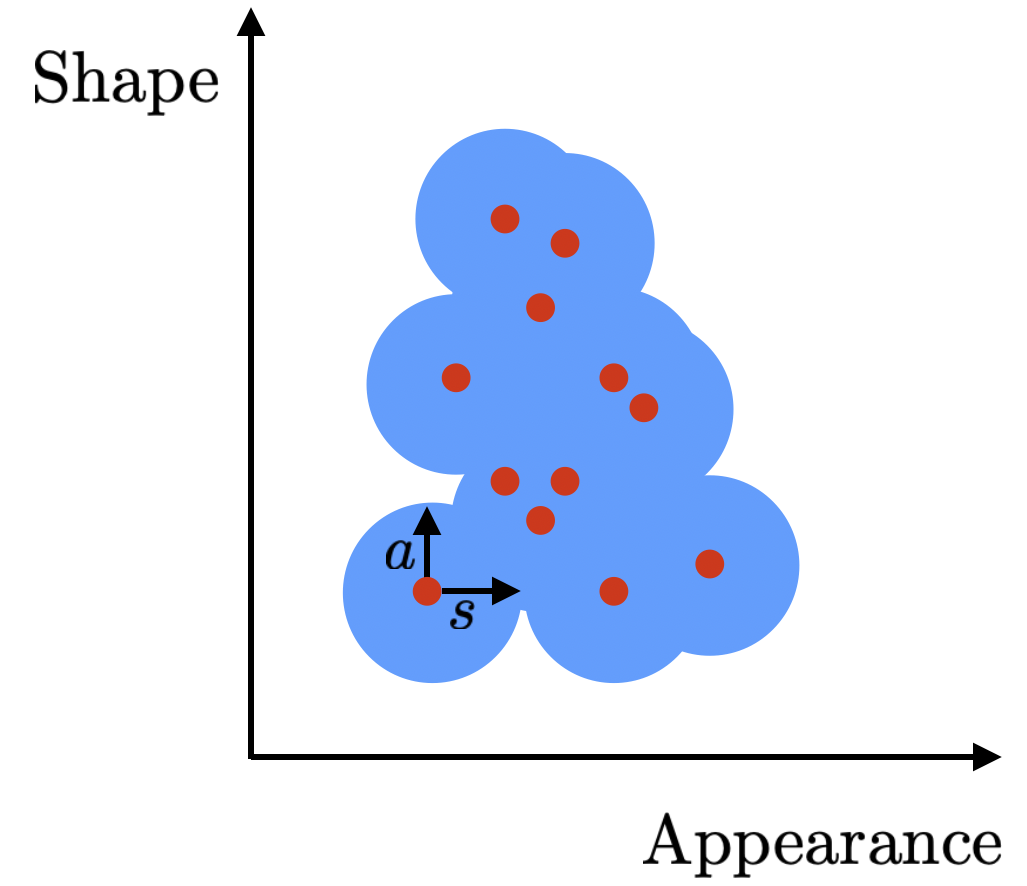
\includegraphics[trim={0cm 0cm 0cm 0cm},clip, width=1.\linewidth]{fig/other/trans2}
				\caption{}
			\end{subfigure}
			\caption{Effect of transformations on data distribution: (a) Data points (red) can be connected via a shape $s$ and an appearance $a$ transformation. (b) Applying transformations effectively blurs the data distribution.}
			\label{fig:trans}
		\end{figure}

		In this section we discuss the effect of the transformations on learning a consistent and comprehensive representation.
		Since strong image transformations can make the learning curve for the algorithm too steep, we exponentially schedule the increase in magnitude, finally resulting in image changes as shown in Fig. \ref{fig:coloraugm}.
		In effect, the transformations teach the algorithm what changes in shape and appearance are. Assuming that samples from the data distribution are related via a change in shape and appearance, the transformations blur the distribution. This data augmentation effect is sketched in Fig. \ref{fig:trans}.

		\subsection{Spatial Transformations}\label{sec:warps}
			We perform thin-plate spline (TPS) warps to mimic spatial transformations. These changes incorporate rotation, scaling and translation as a special case. While irreplaceable for calculating the direct equivariance loss\todo{ reference to equation}, they can result in artificial shape changes. After all, most objects - such as human beings or animals, do not warp, but articulate their parts/limbs.
			Natural shape changes are needed to learn a model of the objects articulation. These changes are presented in video data. Hence, for videos we enforce the reconstruction to function across different frames. This results in a much stabler performance and greater part consistency especially for highly articulated parts such as arms.

		\subsection{Appearance Transformations}
			% COLOR
			\begin{figure}[htp]
				\centering
				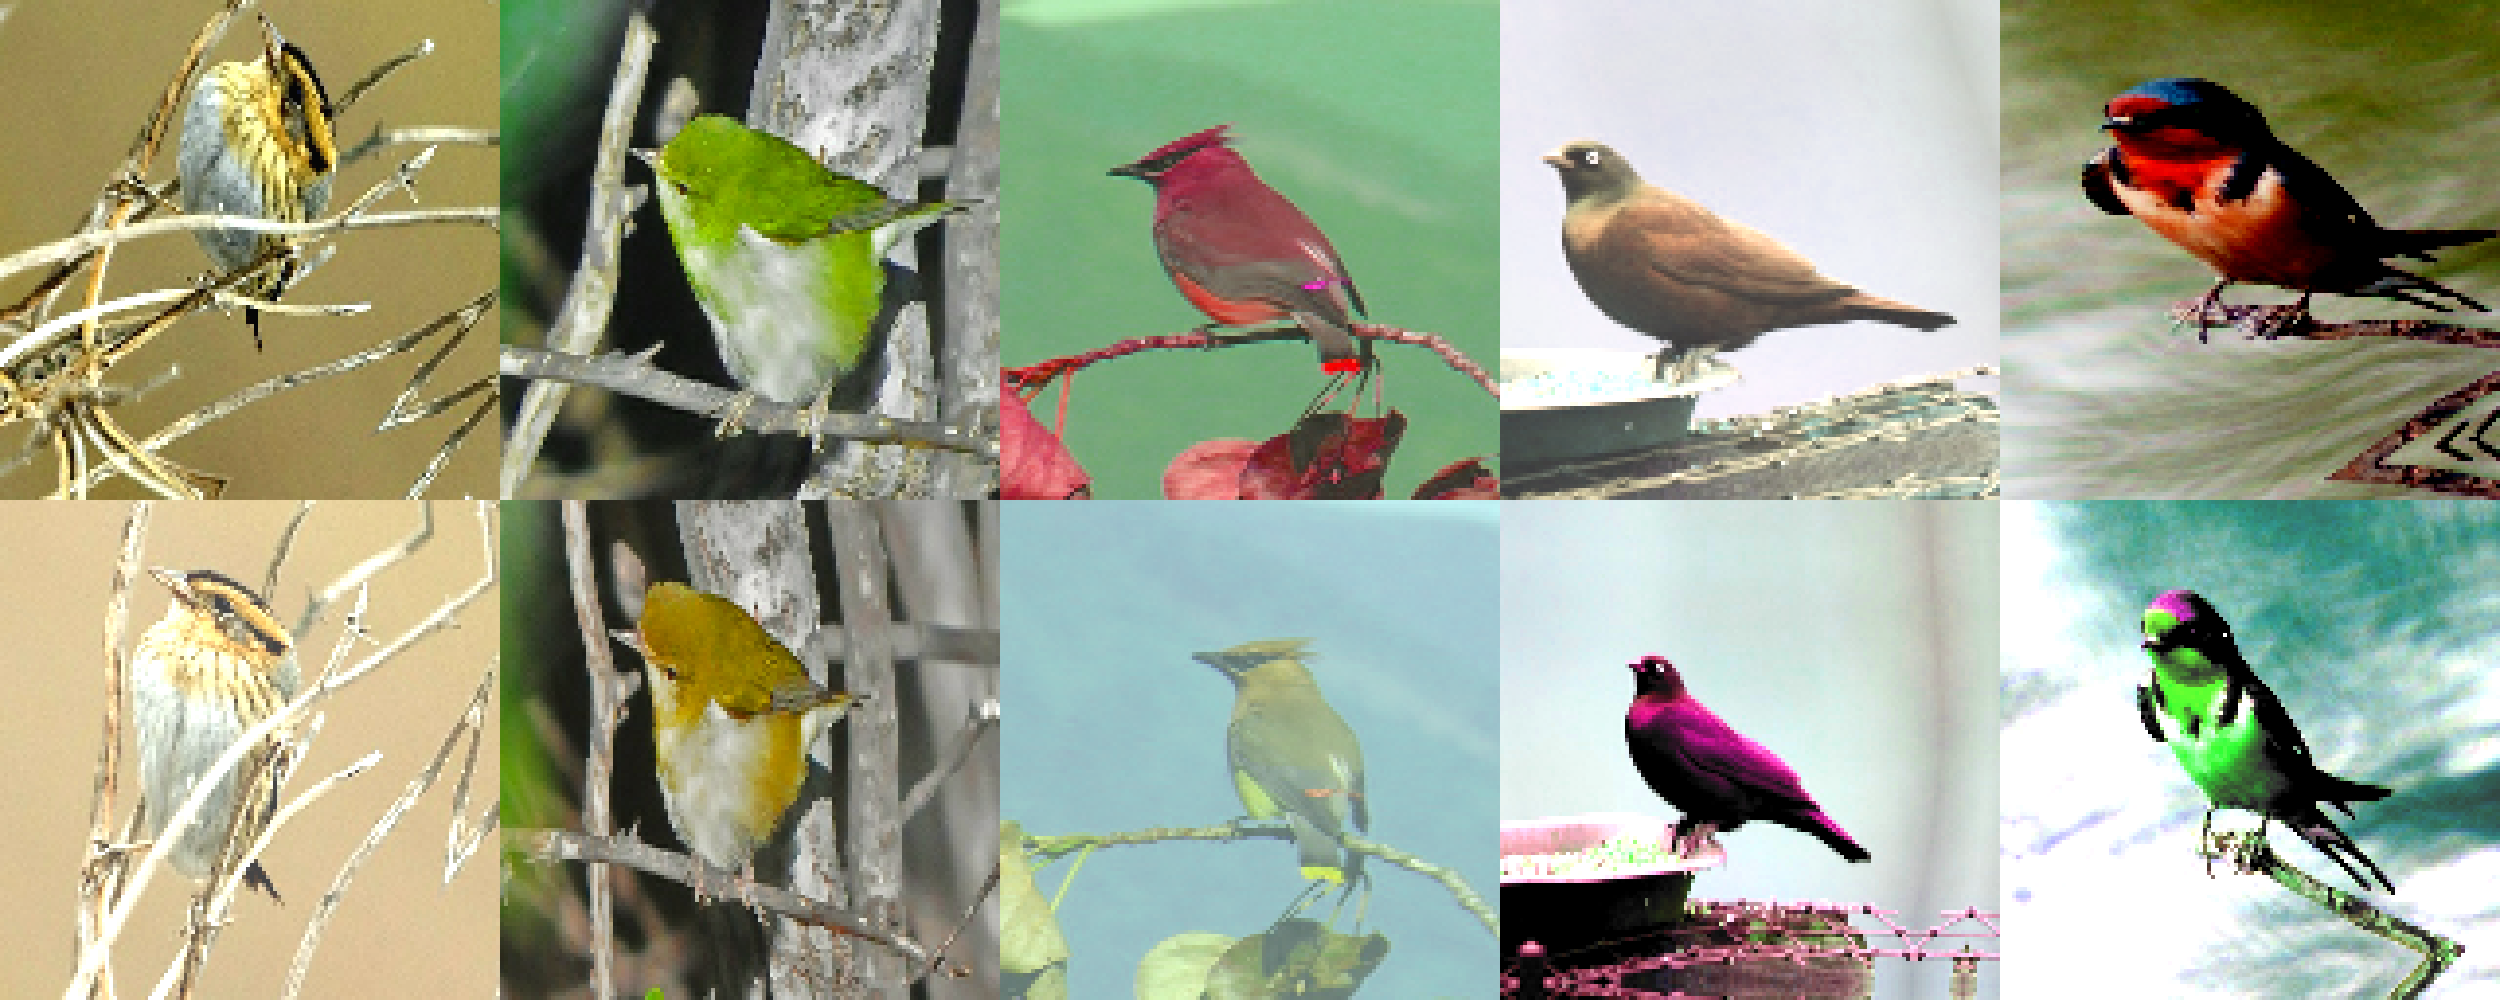
\includegraphics[trim={0cm 0cm 0cm 0cm},clip, width=.8\linewidth]{fig/shape/coloraugm}
				\caption{Examples for shape and appearance transformation on CUB-200-2011. Images from the upper row relate to images directly below.}
				\label{fig:coloraugm}
			\end{figure}

			We mimic appearance changes with image transformations in color, contrast, hue and brightness. Exemplars for the combined effect of spatial and appearance transformations are shown in Fig. \ref{fig:coloraugm}.
			Especially for datasets with high intra-class appearance variance, connecting the data points via appearance changes is crucial. On Cat Head for example, without them, the method assigned different landmarks to black cats than to other-color cats. The model will incur no loss, as long as it always has to reconstruct black cats from images of black cats. If it has to relate black and white cats (\eg via color inversion) this intra-class inconsistency has to vanish.
			Ideally one would want more "natural" appearance changes as well. This could be a line of future work (cf. Sec.~\ref{sec:futurework}).


		\subsection{Parity Transformations}\label{sec:parity}
			\begin{figure}[htp]
				\centering
				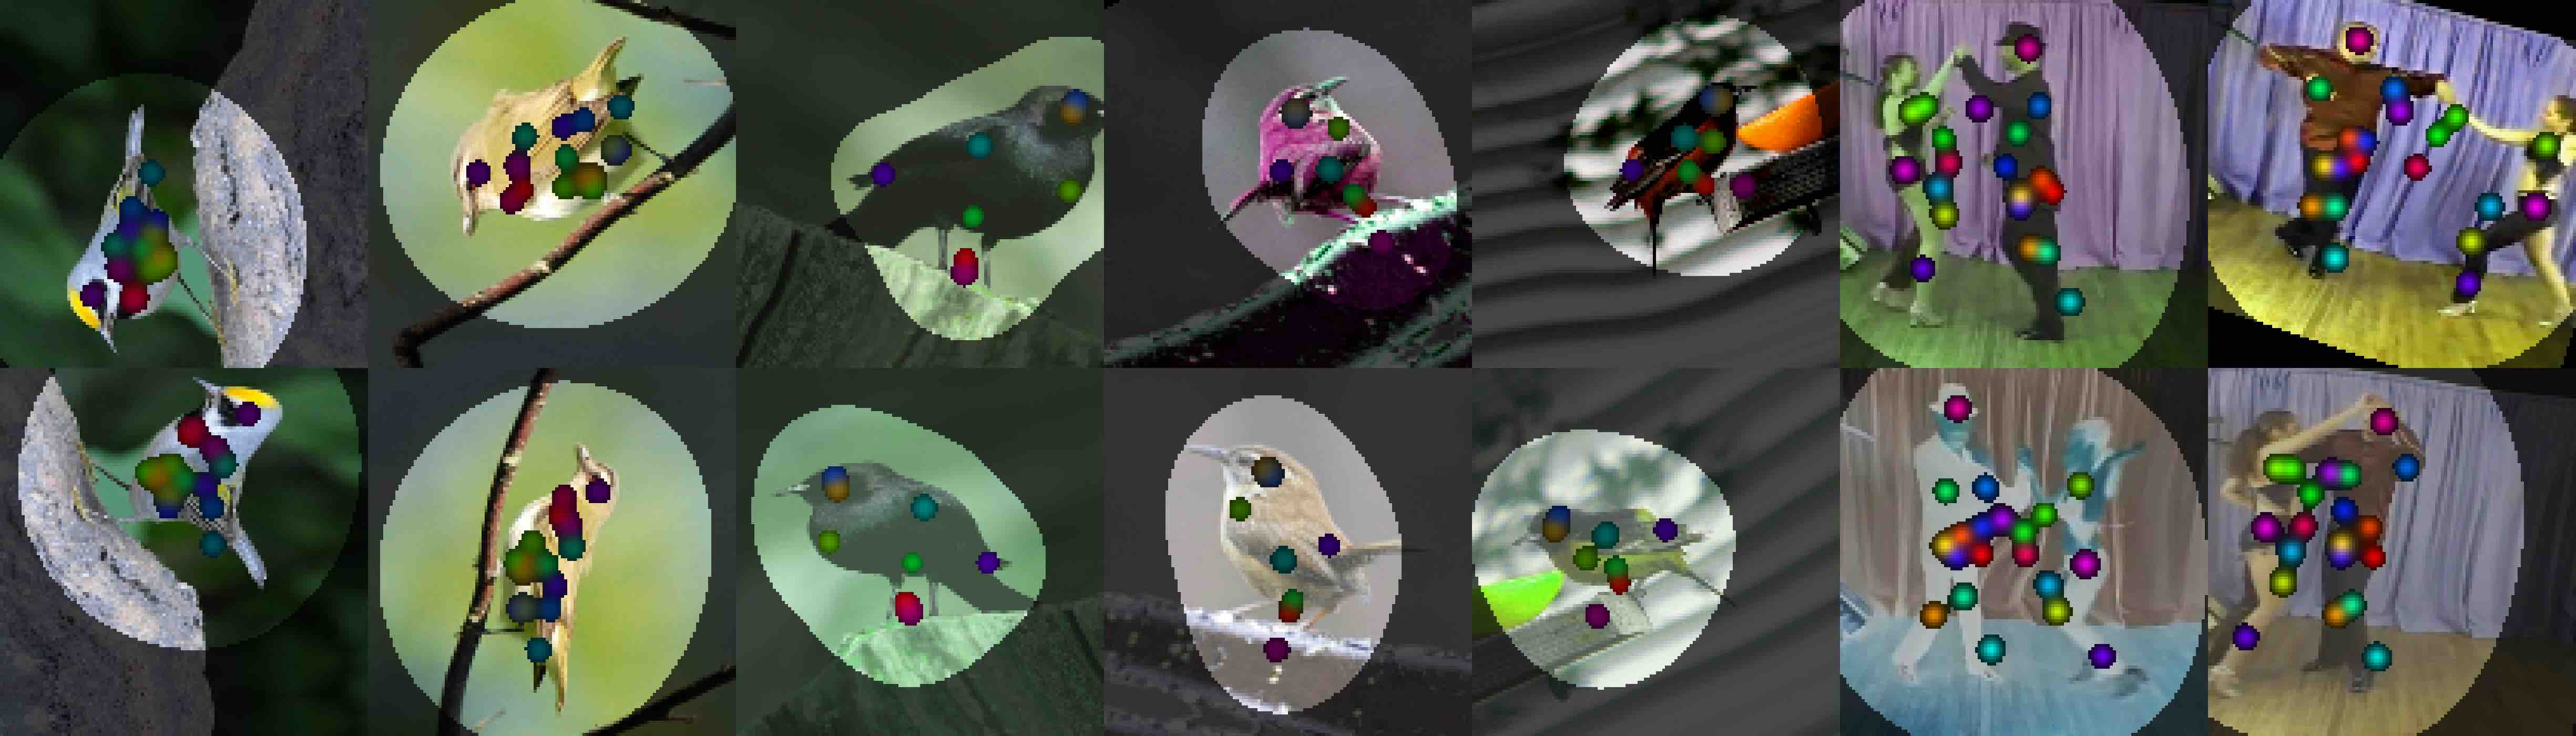
\includegraphics[trim={0cm 0cm 0cm 0cm},clip, width=1.\linewidth]{fig/shape/parity}
				\caption{Parity changes: the images of the upper and lower row relate via the usual transformations and an additional parity flip. For the bird (1-5th column) images induced artificially, for the dancing humans (6-7th column) via sampling different frames from a video.}
				\label{fig:parity}
			\end{figure}
			\todo{make parity failure image}
			The model has problems with consistent part assignment under parity changes, if these changes do not change the object enough. For example human body appearance in frontal and back view are not dissimilar enough from each other. So the model can assign the same landmark to \eg the right arm in the frontal view and the left arm in the back view.
			Similarly, there is no distinction, for dog or bird side views facing to the left or right. However, if features on the left and on the right are very different \eg for the dancing humans the model automatically learns the distinction (see Fig.~\ref{fig:parity}).

			A tentative solution to the problem can be to incorporate parity flips in the equivariance loss. This is impossible for parity-symmetrical objects (such as frontal view humans), but works \eg for side view dogs or birds. One has to be careful in scheduling these random parity flips, as landmarks tend to align along the mirror axis as a trivial solution. A successfully learned parity model for CUB-200-2011 is shown in Fig.~\ref{fig:parity}.

		\subsection{Importance of Transformations}
			The proposed method enables to abstract away object appearance from shape.
			Despite the multifarious challenges in the diverse range of datasets, the method is able to learn a dedicated part representation for shape.
			We compare to other approaches and reach state-of-the-art performance on the task of regressing human-annotated landmarks from the part representation.
			The key difference to the most competitive approach \cite{zhang18} is the emphasis on disentanglement via a crossed reconstruction with shape and appearance transformations.
			Enforcing disentanglement via targeted transformations enhances the shape representation in two ways: \emph{(i)} it asserts that no appearance information is encoded in the shape representation and vice versa and \emph{(ii)} it requires visual features to be equivariant under a spatial transformation.
			With regards to the considerations earlier, the crucial role of the transformations is to be expected, as they enable to reach a \textit{disentanglement}. In the next section we explore and compare the performance on disentanglement.

